% ****** Start of file apssamp.tex ******
%
%   This file is part of the APS files in the REVTeX 4.2 distribution.
%   Version 4.2a of REVTeX, December 2014
%
%   Copyright (c) 2014 The American Physical Society.
%
%   See the REVTeX 4 README file for restrictions and more information.
%
% TeX'ing this file requires that you have AMS-LaTeX 2.0 installed
% as well as the rest of the prerequisites for REVTeX 4.2
%
% See the REVTeX 4 README file
% It also requires running BibTeX. The commands are as follows:
%
%  1)  latex apssamp.tex
%  2)  bibtex apssamp
%  3)  latex apssamp.tex
%  4)  latex apssamp.tex
%
\documentclass[%
 reprint,
%superscriptaddress,
%groupedaddress,
%unsortedaddress,
%runinaddress,
%frontmatterverbose, 
%preprint,
%preprintnumbers,
%nofootinbib,
%nobibnotes,
%bibnotes,
 amsmath,amssymb,
 aps,
%pra,
%prb,
%rmp,
%prstab,
%prstper,
%floatfix,
]{revtex4-2}

\usepackage{graphicx}% Include figure files
\usepackage{dcolumn}% Align table columns on decimal point
\usepackage{bm}% bold math
\usepackage{commath}
\usepackage[hidelinks]{hyperref}
\usepackage{cleveref}
\usepackage{float}

% \usepackage{wrapfig}
% \usepackage[font=small,labelfont=bf]{caption}
% \usepackage{subcaption}
% \usepackage{color}
% \usepackage{listings}
% \usepackage{tabularx}
\usepackage{svg}
% \usepackage{mhchem}

%\usepackage[mathlines]{lineno}% Enable numbering of text and display math
%\linenumbers\relax % Commence numbering lines

% \usepackage[showframe,%Uncomment any one of the following lines to test 
%%scale=0.7, marginratio={1:1, 2:3}, ignoreall,% default settings
%%text={7in,10in},centering,
%%margin=1.5in,
%%total={6.5in,8.75in}, top=1.2in, left=0.9in, includefoot,
%%height=10in,a5paper,hmargin={3cm,0.8in},
%]{geometry}

\begin{document}

\preprint{APS/123-QED}

\title{Percolation Theory:\\an Investigation}% Force line breaks with \\

\author{Oliver Dudgeon}
\author{Adam Shaw}
\author{Joseph Parker}

\date{\today}

\begin{abstract}
An article usually includes an abstract, a concise summary of the work
covered at length in the main body of the article. 
\begin{description}
\item[Usage]
Secondary publications and information retrieval purposes.
\item[Structure]
You may use the \texttt{description} environment to structure your abstract;
use the optional argument of the \verb+\item+ command to give the category of each item. 
\end{description}
\end{abstract}

%\keywords{Suggested keywords}%Use showkeys class option if keyword
                              %display desired
\maketitle

\section{Introduction}
Structure\\
- Generic description of perc theory \cite{stauffer_introduction_2003}\\
* Site and Bond percolation\\
- Areas where it's used\\
    * Epidemic models (COVID-19) \cite{mello_epidemics_2020}\\
- Why investigate further\\
- Report structure\\

\section{Models}
Site percolation on a 2D lattice\\
* How it's generated\\
* What's meant by critical point\\
- hoshen kopelman (HK) clustering algorithm \cite{hoshen_percolation_1976}\\
* Description of algorithm and why it's good\\
* Optimisations and multiprocessing (cluster splitting)\\
* How we optimised (not as useful method)\\
- Flowchart \cref{fig:hk_flow}\\
\begin{figure}
    \centering
    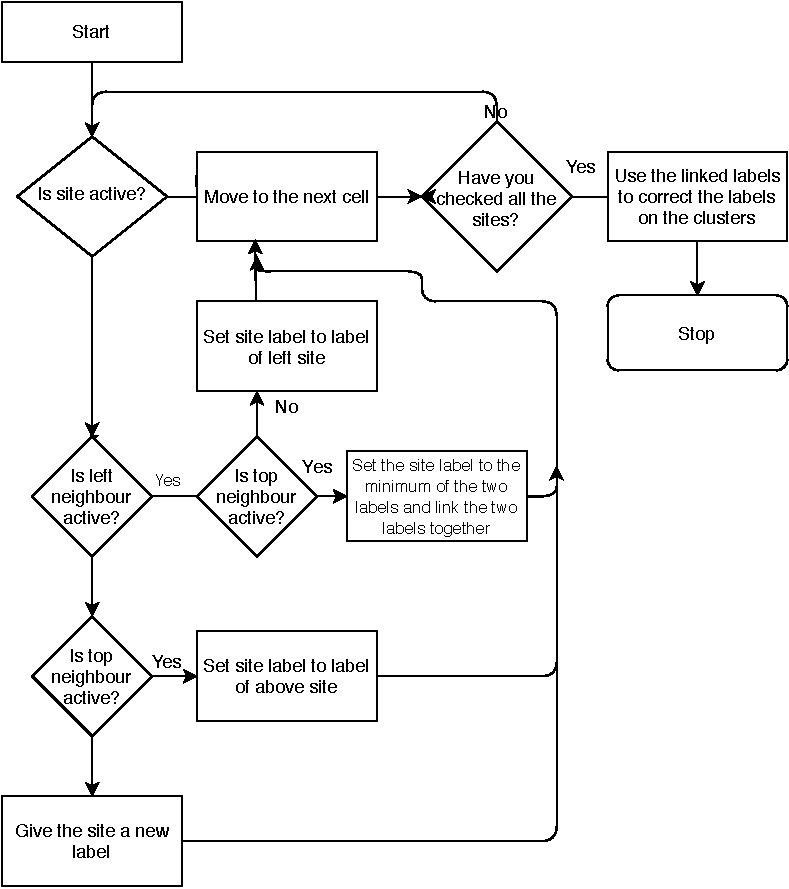
\includegraphics[width=\linewidth]{assets/hk_algroithm}
    \caption{Flowchart}
    \label{fig:hk_flow}
\end{figure}
- SciPy algorithm\\
* The data structure they used\\
* Their choice of algorithm\\
* Why it's faster than ours?\\
- Theory for critical points\\
* Changes in properties at critical point for site perc\\
* What these mean for physical systems\\
* How I found the critical points\\

Forest Fire Model\\
- Theory for critical points\\

\section{Results}

Site\\
- number of clusters\\
* Give reasoning for shape of the curve at three values of p\\
* Link into polyminoes\\
- polyminoes\\
* What is a polymino
- critical probability\\
* Show results from critical probability 
* Introduce plots\\
* Identify critical point on graph\\
* Calculate critical exponents from graph
- Weird graph?
* Understand what's going on physically
* Describe why this may be of importance

FF\\
- Gifs
- 

\section{Discussion}

\section{Conclusion}

\bibliography{apssamp}% Produces the bibliography via BibTeX.

\end{document}
%
% ****** End of file apssamp.tex ******
